\documentclass[tikz,border=10pt]{standalone}
\usepackage{ctex} % 如需中文支持
\usetikzlibrary{calc}

\begin{document}

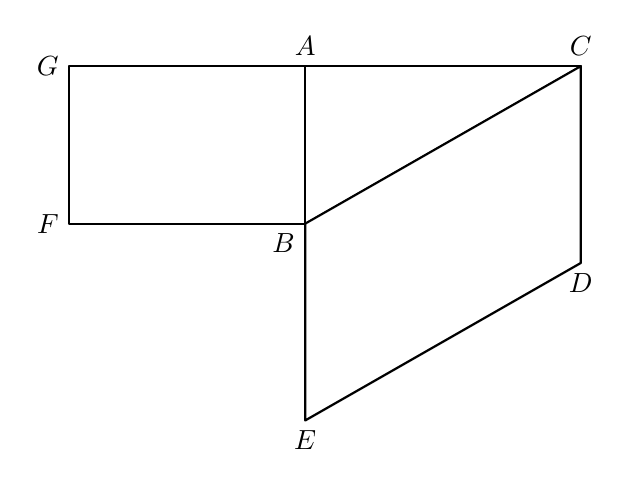
\begin{tikzpicture}[line cap=round, line join=round, >=stealth, thick]
    % --- 参数定义 ---
    \def\rectW{3}  % 左侧矩形的宽度 (G-A)
    \def\rectH{2}  % 左侧矩形的高度 (G-F)
    \def\paraW{3.5} % 右侧平行四边形的水平跨度 (A-C)
    \def\paraH{2.5} % 右侧平行四边形的垂直跨度 (B-E)

    % --- 坐标点定义 ---
    % 以 A 点为原点 (0,0)
    \coordinate (A) at (0,0);
    \coordinate (G) at (-\rectW, 0);
    \coordinate (B) at (0, -\rectH);
    \coordinate (F) at (-\rectW, -\rectH);
    
    \coordinate (C) at (\paraW, 0);
    \coordinate (E) at (0, {-\rectH-\paraH});
    % 计算 D 点：使得 BCDE 为平行四边形 (D = C + (E-B))
    \coordinate (D) at ($ (C) + (0, -\paraH) $);

    % --- 绘制图形 ---
    % 1. 绘制左侧矩形 ABFG
    \draw (G) -- (A) -- (B) -- (F) -- cycle;
    
    % 2. 绘制右侧图形 BCDE
    \draw (B) -- (C) -- (D) -- (E) -- cycle;
    
    % 3. 补充连接线 (由图可见 AC 是一条直线段)
    \draw (A) -- (C);

    % --- 标注顶点标签 ---
    % 这里的 anchor 参数用于调整文字相对于点的位置，确保不被线遮挡
    \node [above] at (A) {$A$};
    \node [below left] at (B) {$B$};
    \node [above] at (C) {$C$};
    \node [below] at (D) {$D$};
    \node [below] at (E) {$E$};
    \node [left] at (F) {$F$};
    \node [left] at (G) {$G$};

\end{tikzpicture}

\end{document}